\chapter[Rethinking Resampling Methods]{Rethinking Resampling Methods: Random Is Not Unbiased} \label{ch4:resampling}
\chaptermark{Rethinking Resampling Methods}
\setlength{\epigraphwidth}{4.5in}
\epigraph{If two things are similar, the thought of one will tend to trigger the thought of the other.}{Aristotle, \textit{``Laws of Association''}, 300 B.C.}

%----------------------------------------------------------------------------------------------------------------------------------------------------------------------------------------------------------
\section*{Summary}
After a statistical learning method is chosen and applied, the model needs to be tested. Most statistical learning techniques used in water resources modeling employ a randomized splitting of data into k-folds to estimate model error. In each iteration, one fold is held out as a test set and others are designated as a training set. Such random cross-validation methods ignore structures in the data, which underestimate model error  \cite{roberts2017cross}. % Also, models evaluated with randomized cross-validation methods disregard the assumption of independence of residuals. When mapping the residuals in time or in space, the trends point to dependence structures in the data that produce an over-fit model with non-causal parameters or missed meaningful parameters. %cite?

A more accurate estimate of the model error can come from techniques that block training sets in time, space, or unique structure (e.g., by hydrologic basins). The difficulty here lies in specifying block sizes in time and space. Blocking potentially reduces the range of parameters seen by the model, or may exclude a particular meaningful combination of predictor variables in the training data set. Too small of a block size and the cross-validation method more closely mimics the randomized method and runs the risk of under estimating model error. Large block sizes force too much model extrapolation and risk over estimating model errors. 

This chapter compares resubstitution, Monte Carlo (i.e., randomized), leave one group out (LOGO), and leave multiple groups out (LMGO) cross-validation strategies, as well as, resubstitution, Monte Carlo, blocked by group (BBG), blocked by multiple group (BBMG), and blocked by hierarchy (BBH) bootstrapping strategies for modeling synthetic unimpaired flows. This chapter intends to assess the sensitivity of the estimated uncertainty to the aforementioned resampling methods. 
%The resubstitution and random methods least accurately, and the LMGO method most accurately estimate the error in the Random Forest model (a regression tree based statistical learning algorithm). 

%----------------------------------------------------------------------------------------------------------------------------------------------------------------------------------------------------------
\section{Introduction} \label{ch5:introduction}
% add literature review here
% the data
Most, if not all, geographic data have internal correlation and dependence structures \cite{legendre1993spatial}: (1) temporal autocorrelation: nature responds to changes gradually. For example, today's precipitation is correlated with yesterday's precipitation; (2) spatial autocorrelation: nearby things tend to be more related than those far from one another. For example, two points close together on a topographic map are likely to have similar elevations;  and (3) hierarchical structures: the network of streams flowing into one another (or more formally, the stream order) provides a hierarchical structure. That is, basin topology provides a spatial structure more complicated than merely proximity of river gauges. For example, two points on a river may be close in proximity but depending on which side of the watershed divide they fall on they can be fed by two different basins, in different hierarchies in the network, with different governing hydrologic processes, and therefore, have different measured flows (See Figure \ref{fig:structured}). 

%(3) groupings: basins provide a spatial structure more complicated than merely proximity of river gauges. For example, two points on a river may be close in proximity but depending on which side of the watershed divide they fall on be fed by two different basins with different governing hydrologic processes, and therefore, have different measured flows; (4) For example, two river points in the same larger basin can be in different hierarchies and subbasins depending on where in the network they lie.

\begin{figure}[ht]
	\centering
	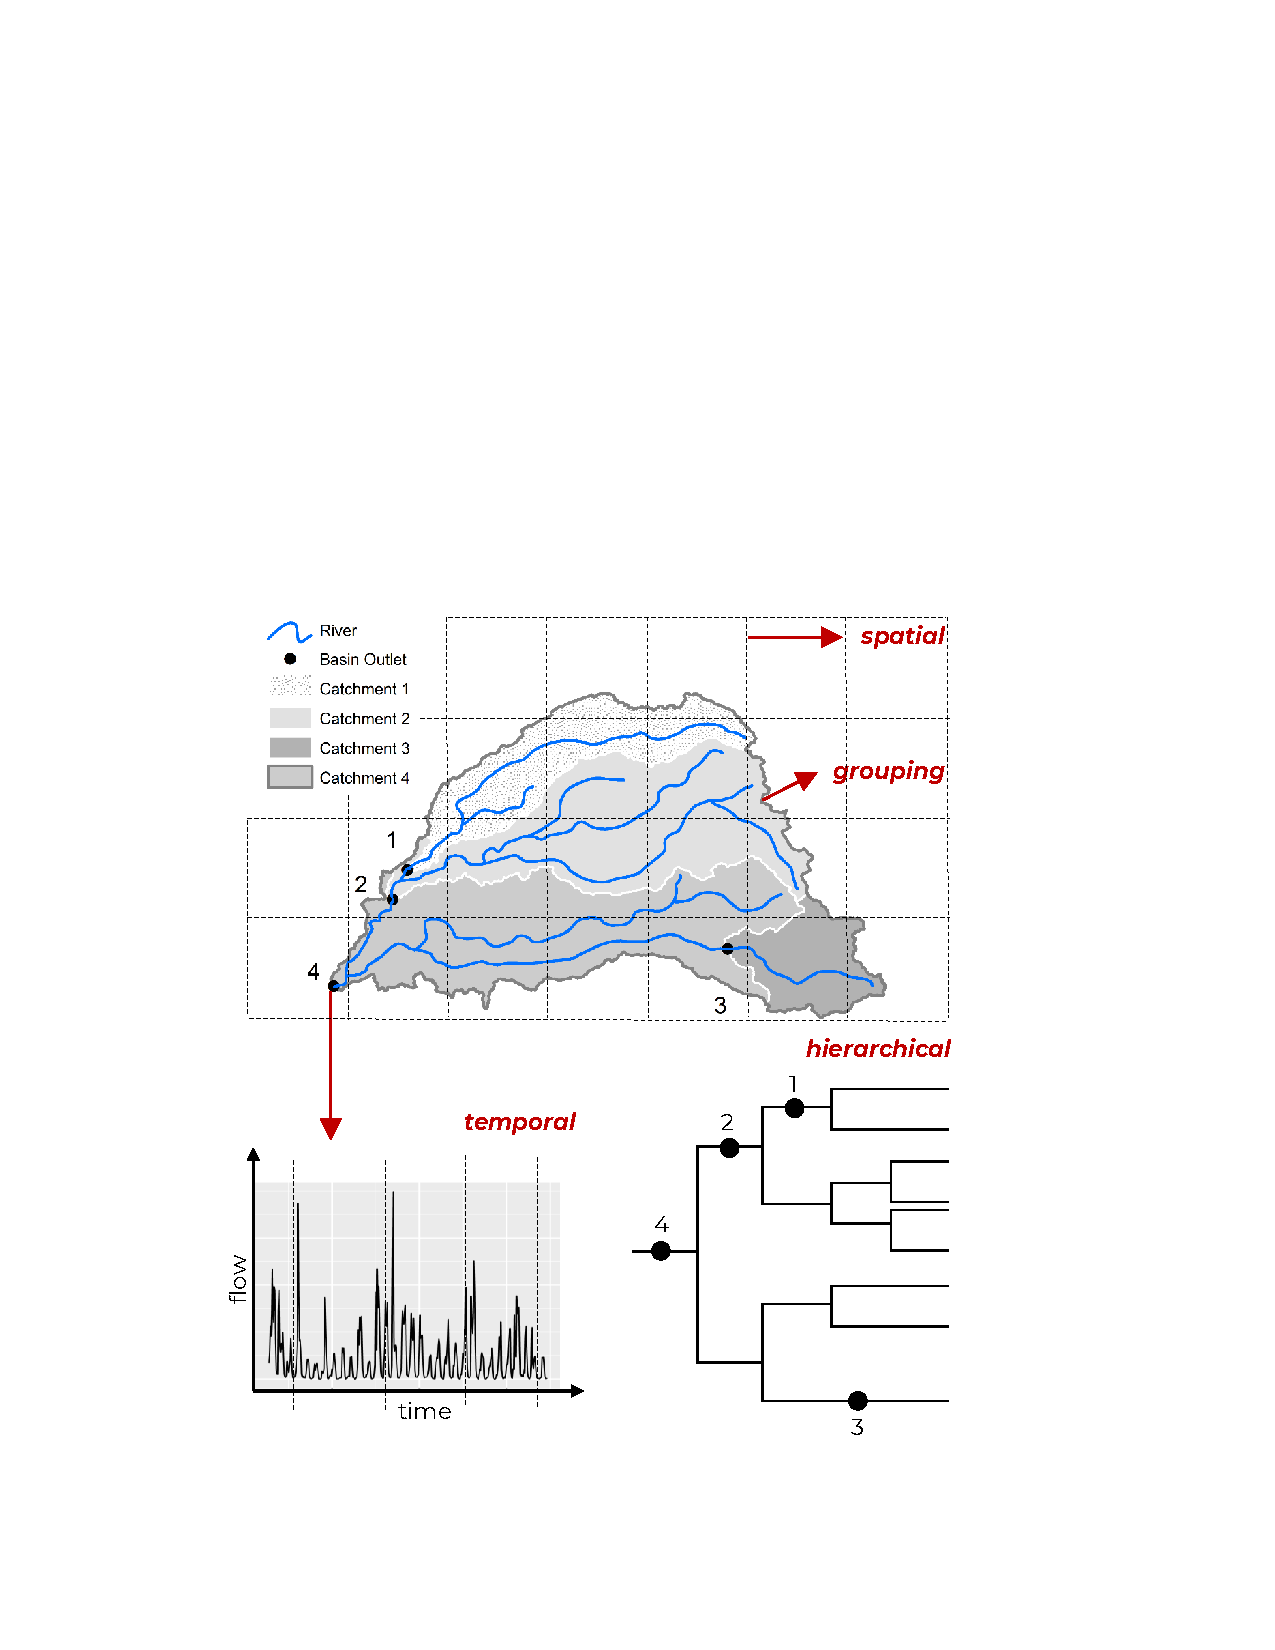
\includegraphics[width=18cm,trim={2cm 3.2cm 0 10.2cm},clip=true]{plots/structured.pdf}
	\caption{The four types of dependence structures in gauged data and blocking strategies} 
	\label{fig:structured}
\end{figure}

% the CV methods? INCLUDE BOOTSTRAP HERE TOO, AND BLOCKING BOOTSTRAP
In predictive modeling, the goal is to accurately predict data, with structures mentioned above, at unmeasured locations either in the past in locations not gauged, or in the future where observations do not yet exist. Therefore, the predictive accuracy of the \textit{training set}, the data the model is trained on, is of little consequence. The \textit{test set} error, the error of a set of data not seen by the model, is the true measure of model accuracy. 

Moreover, the predictive accuracy of the model on the training set can severely differ from the test set. With increasing model complexity (e.g., adding parameters to the model), clearly the model will fit the training data increasingly well. However, errors in the test set behave differently as is evident in the characteristic U-shape of the bias-variance tradeoff curve \cite{friedman2001elements}. The expected error in the test set is a polynomial of power two (See Equation \ref{eq:bvt}) and is comprised of variance, bias, and a constant term. In the first portion of the U, bias will decrease more than the gain in variance, however, past some point, we are now overfitting and the gain in variance is too much to be offset by the decrease in bias. Therefore, depending on how we specify the model, we will lie somewhere along this U shape and cannot substitute training error rates for the true predictive capability of the model. 

The test set error can be easily calculated if such a data set exists, or, it can be estimated by holding out a subset of the training data. The holding-out is achieved by resampling strategies, to effectively creating a test set. Two resampling methods are: \textit{cross-validation} and \textit{bootstrapping}. In cross-validation, the data set is split into testing and training data sets where each observational unit gets a chance at being in the test set once. In bootstrapping, sampling is done with replacement where each observational unit gets an equal chance at being selected and being selected more than once. In this case, on average 1/3\textsuperscript{rd} of the data set will end up not being selected at all, in other words these observations are out-of-bag \cite{efron1997improvements}. 

With the test set, that is held out observed data, and our model's results, we can conveniently apply any statistical measure of fit desired as a proxy for model accuracy (e.g., Nash-Sutcliffe Efficiency (NSE)). 

% the problem
Most studies, in water resources, ignore dependence structures in the data when devising a resampling strategy. When testing data are randomly selected from the entire spatial domain, training and testing data from nearby locations will be dependent due to \textit{spatial autocorrelation}. Therefore, if the objective is to project outside the spatial structure of the training data (e.g., to an ungauged basin), error estimates from random cross-validations or the bootstrap statistic, will be overly optimistic \cite{roberts2017cross}. 

% NOT RELEVANT HERE, MAKE A NEW CHAPTER MAYBE?
% Most studies, also fail to examine the autocorrelation of the errors produced by the developed models; as such, inferential results can be biased. Either including additional predictor variables, or choosing a different functional form has to be considered if a strong autocorrelation is detected in the model's residuals. The problem of inference cannot be diagnosed without explicitly checking for the spatial and temporal variability of the residuals, which are supposed to be independent and not correlated. A simple visual check or a formal test of the significance of Moran's I or Geary's C can help in this regard. 

In essence, a correlation structure points to a pseudo replication problem (See Figure \ref{fig:marbles}). For $x^d$ at a distance, $\Delta d$, from $x^{d+\Delta d}$, where $x^d$ and $x^{d+\Delta d}$ are autocorrelated. The distance $\Delta d$ can be defined in time, space, or hierarchy. In random resampling, either of the autocorrelated values may lie in the bag of samples given to the model, or it may be left out-of-bag. Therefore, the model can easily predict one, given that the other is likely in the bag. However, in blocking resampling the two observations are connected and will both end up in the bag or out-of-bag. Here, the model is forced to predict a phenomenon from other observations. 

\begin{figure}[ht]
	\centering
	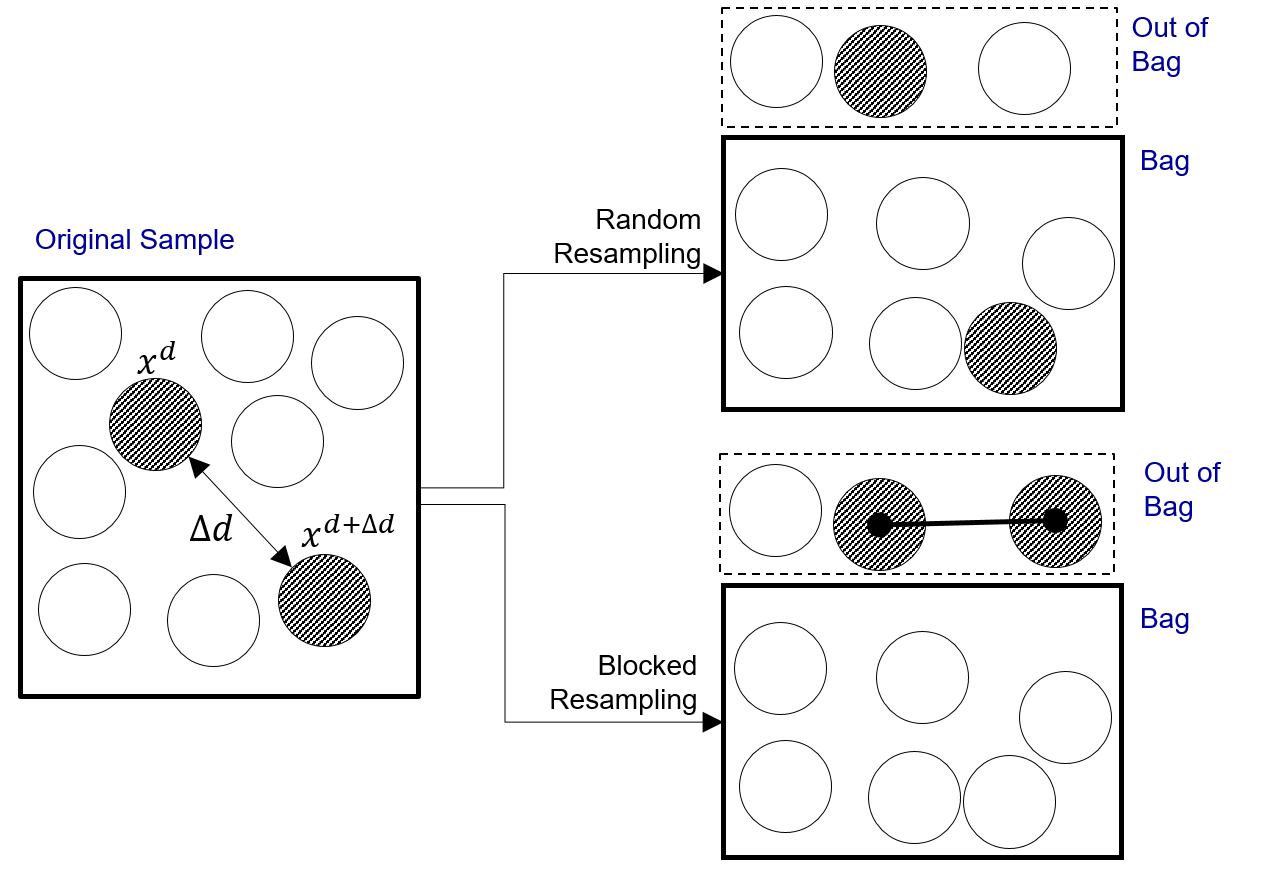
\includegraphics[width=15cm,trim={0 0 0 0},clip=true]{plots/resampling.png}
	\caption{Autocorrelation is a pseudo replication problem. The two grey marbles are autocorrelated. A model that uses random resampling will be able to easily predict one grey marble since it has seen the other. When blocking, the observations move in and out of the bag together.} 
	\label{fig:marbles}
\end{figure}

% Why bother? 
While correlation structures may not be as problematic in conventional statistics, combined with high-dimensions and low sample sizes, predictive methods suffer. Compounding the problem can be low computational abilities (See Figure \ref{fig:blocksizes}).

\begin{figure}
	\centering
	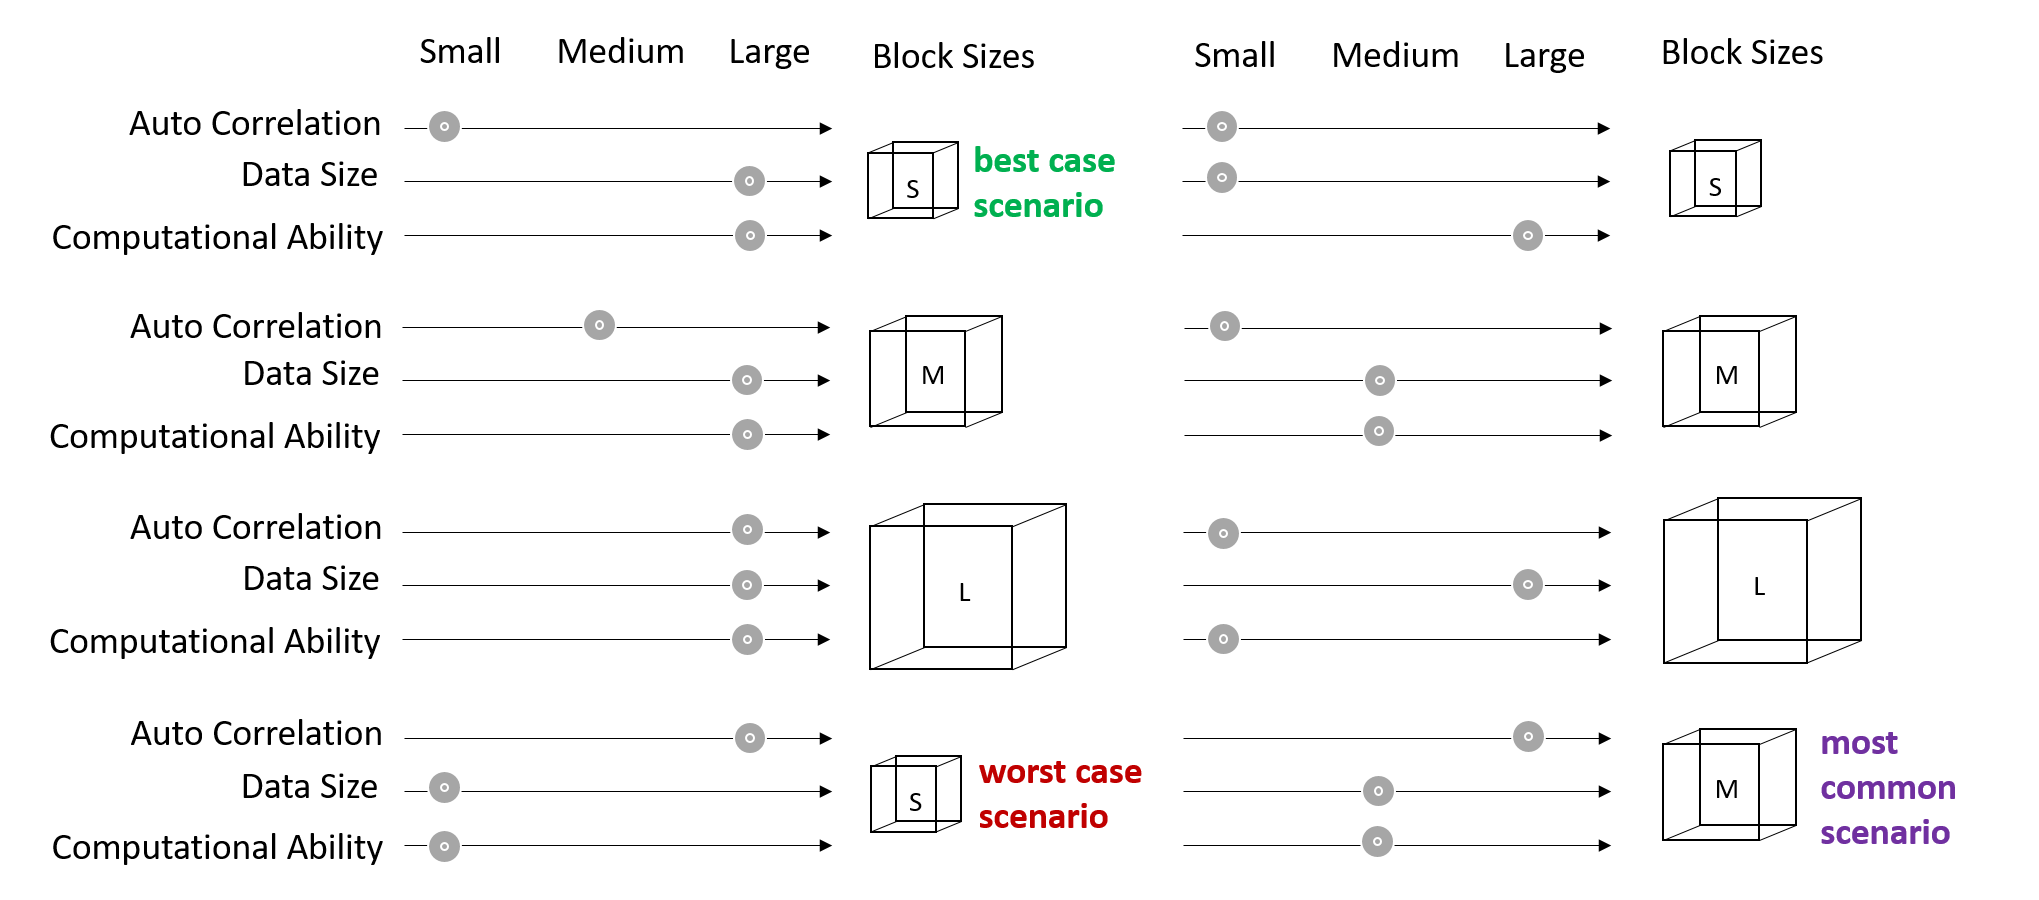
\includegraphics[width=15cm,trim={0 0 0 0},clip=true]{plots/blocksizes.png}
	\caption{The block size in resampling methods is a function of the autocorrelation, data size, and computational ability.} 
	\label{fig:blocksizes}
\end{figure}

%-----------------------------------------------------------------------------------------------------------------------------------------------------------------------------------------------------
\section{Research Design} \label{ch5:design}
Resampling methods are generally used to either: (1) estimate the accuracy of sample statistics (e.g., the standard deviation of an $\alpha$ parameter in a linear model $y=\alpha x+\beta$); (2) estimate the accuracy of significance tests (e.g., p-values); or (3) test the models. In hydrology, when examining observed data, the true population (i.e., the set of all possible hydrologic states) is unknown and the true error in the model or a sample statistic is unknowable. Therefore, we commonly use resampling methods to test our model's predictions. 
%In this case, our models will be performing quite differently from one another because of the differences in training and testing splitting strategies, which will be explained later. 
% To some extent, the modeling method follows that outlined in \cite{roberts2017cross}. 

In this study, data from a mechanistic simulation model, the Basin Characterization Model (BCM), with fitted values are considered as ``true" unimpaired flows. The BCM approximates California hydrology well. It estimates monthly unimpaired flows and is developed and maintained by the U.S. Geological Survey (USGS). The data spans California at 270m x 270m resolution. The recharge and runoff estimates from the BCM are attained from physically based equations that calculate potential evapotranspiration, snow, excess water, and actual evapotranspiration. Depending on soil properties and the permeability of underlying bedrock, surface water can be classified for each cell as either recharge or runoff \cite{flint2014california}. 

The recharge and runoff rasters can be aggregated to any given basin. Here, the machine learning model will be trained on the simulated runoff values from the BCM aggregated to the CDEC basins (See Figure \ref{fig:map}). The developed data set has approximately 18,500 monthly unimpaired flow observations in acre-feet (AF) (See appendix \ref{f:bcmdata} for more info). The data spans from 1895 to 2018 at a monthly time step. As mentioned in Chapter \ref{ch3:guide}, we will develop a GLM, RNN, and TMARS model. That said, the focus of this study is to demonstrate the differences between the cross-validation methods, not on the data or the machine learning method themselves; the purpose is to see which resampling strategy used in the machine learning algorithm gives the closest estimate to the true model error. That is, we want to see which cross-validation or bootstrap method is most appropriate for the machine learning model predicting values of a known model. In this chapter, we considered MSE as the loss function and the model measure of fit (See Equation \ref{eq:mse}).

To find the MSE of the machine learning technique: (1) simulate $n$ landscapes of the data by resampling the original data set using the bootstrap method (resampling with substitution); (2) separate the data into training and testing sets (use the CV or BS methods discussed below); (3) for each simulation feed the training data into the desired machine learning algorithm (i.e., a GLM, RNN and TMARS); (4) calculate the desired model measure of fit for each of the simulations; and (5) compare the Probability Density Function's (PDFs) of the model measures of fit with an ``ideal" one (See Figure \ref{fig:bsmethods} \&\ref{fig:cvmethods}).   

In both the cross-validation and bootstrap, the resampling results are compared to an ``ideal'' MSE, which was calculated by: (1) producing one model for each simulated landscape; (2) using said model to predict to the other $n-1$ landscapes; (3) using the predicted and observed values to calculate the MSE for each $n-1$ landscape; (4) averaging the MSE of the $n-1$ landscapes; (5) repeating the process for all $n$ landscapes; and (6) resulting in $n$ MSEs, one for each landscape, which can be plotted as a PDF (See Figure \ref{fig:idealmethod}). 

% can use a parametric bootstrap, but explain the high dimensionality of the problem
\begin{figure}[ht]
	\centering
	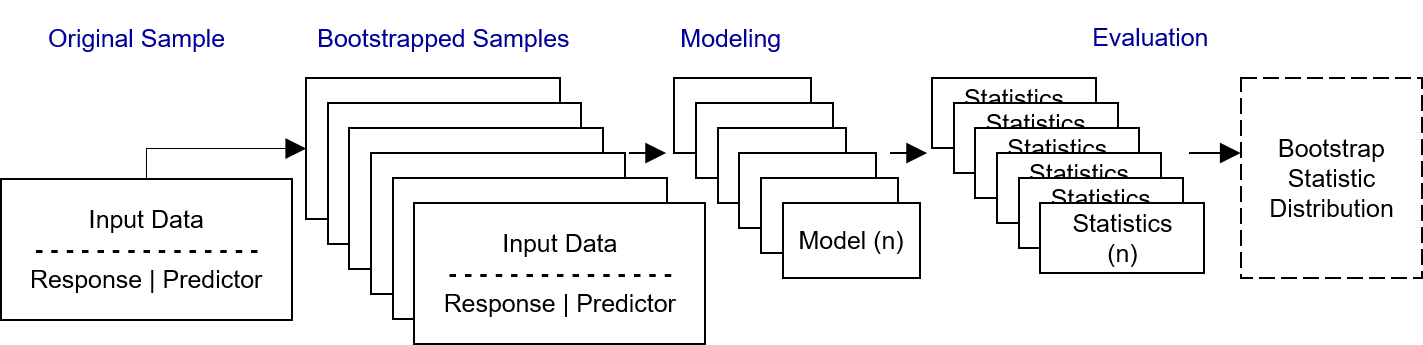
\includegraphics[width=15cm,trim={0 0 0 0},clip=true]{plots/bs_flowchart.png}
	\caption{Research design: We employ the bootstrap method to find the distribution of the bootstrap statistic.} 
	\label{fig:bsmethods}
\end{figure}

\begin{figure}[ht]
	\centering
	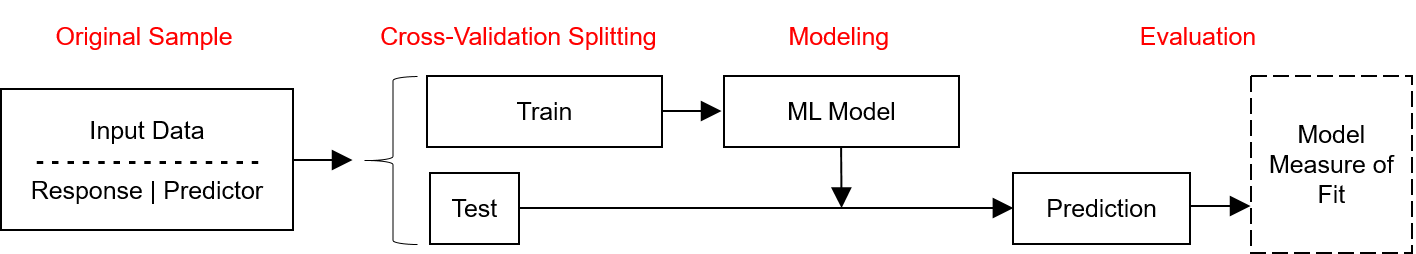
\includegraphics[width=15cm,trim={0 0 0 0},clip=true]{plots/cv_flowchart.png}
	\caption{Research design: We employ the cross-validation method to find the model error estimate.} 
	\label{fig:cvmethods}
\end{figure}

\begin{figure}[ht]
	\centering
	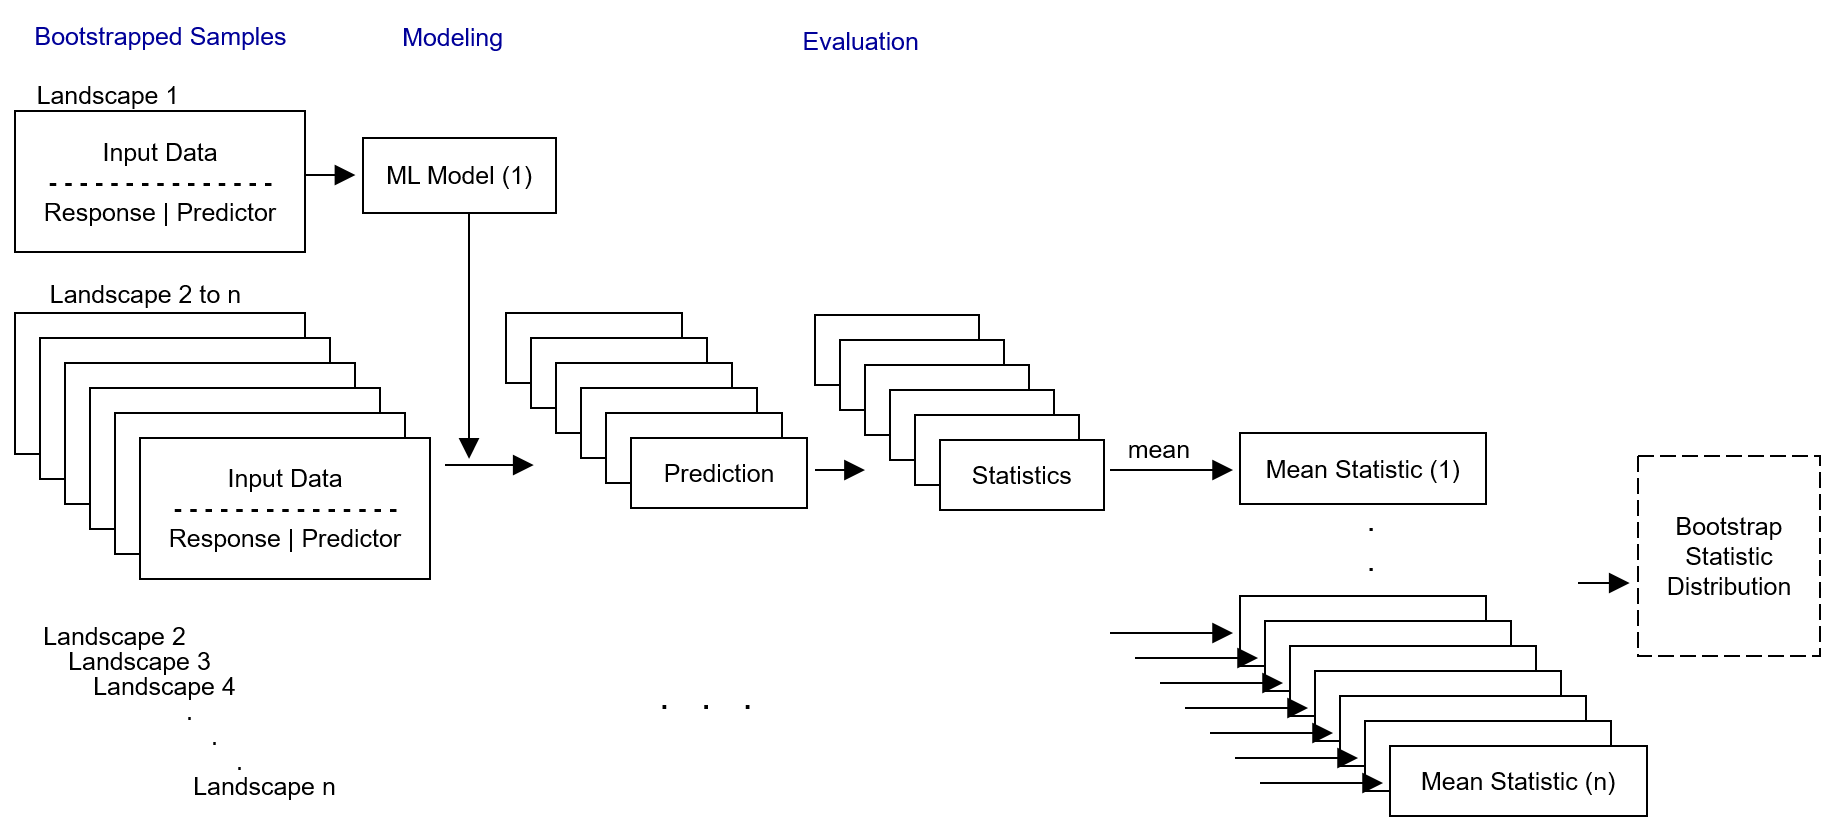
\includegraphics[width=15cm,trim={0 0 0 0},clip=true]{plots/ideal_flowchart.png}
	\caption{Research design: compare the errors with that of an ``ideal" model.} 
	\label{fig:idealmethod}
\end{figure}

%-----------------------------------------------------------------------------------------------
\subsubsection*{Resampling Methods} \label{ch5:resamp}
The second step in the methods mentioned above, separating the data in to training and testing sets, can be accomplished by one of the following methods: 

%---------------------------------------------
\textbf{Cross-Validation}
\begin{itemize}
	\item Resubstitution: the test set is the training set. Here, the model is evaluated against the same data it has already seen. We expect the model to perform the best here and the PDF of the residuals to be closest to 0. 
	\item Randomized or Monte-Carlo:cross-validation
		\subitem Validation Set: the test set is a random 1/2 of the full data set. the training set is the other 1/2. This method is run twice, once with the first half as a test set and next with the second half being the test set. 
		\subitem 5-Fold: the data is split into 5 folds. In each iteration each fold is considered the test set and the other 4 folds the training set. 
		\subitem 10-Fold: the data is split into 10 folds. In each iteration each fold is considered the test set and the other 9 folds the training set. 
	\item Leave One Out (LOO): in each iteration, one instance of the data is help out, and the rest of the data set is the training set. most intense computationally.
	\item Leave One Group Out (LOGO): in each iteration, one basin's data is held out as a whole and the rest of the basins become the training set. The process is repeated for each basin. 
	\item Leave Multiple Groups Out (LMGO): in each iteration, 1/5\textsuperscript{th} or 1/10\textsuperscript{th} of the basin's are held out and the rest of the basins become the training set. The process is repeated for each fold. 
	\item Leave Hierarchies Out (LHO): blocking is design across similar stream orders. %Because of the limitations imposed by datasize we have not considered this cross-validation strategy in this experiment. 
\end{itemize}

%------------------------------------------------
\textbf{Bootstrap Methods}
\begin{itemize}
	\item Resubstitution: same as above, the test set is the training set.
	\item Randomized or Monte-Carlo: the most popular form of bootstrapping where a new data set is built from randomly resampling the original sample with substitution. The length of the data set is the original length of the data set.
	\item Blocked By Group (BBG): the data set is blocked by unique basins. The basins are randomly resampled with substitution. Since the basins may have differing record lengths, the length of the data set may not match the original data set. However, the data set will have the same number of basins as in the original data set. 
	\item Blocked By Multiple Groups (BBMG): the data set is blocked by multiple basins. The grouped basins are randomly resampled with substitution. As the group sizes become larger the blocking size becomes larger. 
	\item Blocked By Hierarchy (BBH): the data set is blocked by stream order. The grouped basins are randomly resampled with substitution. Some stream orders have a chance of occurring in the data set twice where some are left out. 
\end{itemize}

%-----------------------------------------------------------------------------------------------------------------------------------------------------------------------------------------------------
%\section{Preliminary Results} \label{ch5:results}
%True and estimated test MSE for the simulated data sets. PDF of residuals. 
%
%Results show that ignoring the dependence structures when devising testing and training sets produces artificially low errors (See Figure \ref{fig:density}). Here, the resubstitution and randomly drawn folds show lower errors than the blocking methods LOGO and LMGO K-Fold. 
%
%\begin{figure}
%	\centering
%	\begin{subfigure}{.5\textwidth}
%  		\centering
% 		 \includegraphics[width=\textwidth, trim={0 0 0 0}, clip=true]{plots/Rplot22_density_ae.png}
%  		\caption{The error in unimpaired flow. Results are for one simulation. \\}
%  		\label{fig:errorpdf}
%	\end{subfigure}% 
%	\begin{subfigure}{.5\textwidth}
%  		\centering
%  		\includegraphics[width=\textwidth, trim={0 0 0 0}, clip=true]{plots/Rplot24_density.png}
%  		\caption{The model RMSEs for each cross-validation method. Results are across the 25 simulations.}
%  		\label{fig:rmsepdf}
%	\end{subfigure}
%	\caption{PDFs of model error.}
%	\label{fig:density}
%\end{figure}
%
%% Results also show that the size of the blocks matter. The validation set approach most accurately predicts the model error, then the Random 5-Fold, the Random10-Fold and the Resubstitution CV methods. Same phenomenon exists in grouping blocking method: the 5-Fold LOGO most accurately predicts the model error, then the 10-Fold LOGO, the LOGO method and the Resubstitution method. 
%
%\begin{figure}
%	\centering
%	\begin{subfigure}{.5\textwidth}
%  		\centering
% 		 \includegraphics[width=\textwidth, trim={0 0 0 0}, clip=true]{plots/Rplot20_r2map_wrong.png}
%  		\caption{Random 5-Fold CV.}
%  		\label{fig:random5fold}
%	\end{subfigure}% 
%	\begin{subfigure}{.5\textwidth}
%  		\centering
%  		\includegraphics[width=\textwidth, trim={0 0 0 0}, clip=true]{plots/Rplot20_r2map.png}
%  		\caption{LOGO CV.}
%  		\label{fig:logocv}
%	\end{subfigure}
%	\caption{Random 5-Fold CV gives deceptively high R\textsuperscript{2} model fit values.}
%	\label{fig:spatialcvperformance}
%\end{figure}
%
%% The spatial variability. Put the maps of Cali side by side. use the mean of the nsim RMSE values as the point. do this for resub, random 5 fold, and logo only. (See Figure \ref{fig:spatialcvperformance}). Shows we still haven't gotten rid of the spatial autocorrelation!

%-----------------------------------------------------------------------------------------------------------------------------------------------------------------------------------------------------
\section{Conclusion} \label{ch5:conclusion}
This chapter presents various blocking resampling techniques where the observations in a block are bonded together. The idea behind blocked resampling is simple: \textit{birds of a feather flock together}, or more accurately birds of a feather \textit{should} flock together. That is, if two observations are autocorrelated they should be both included in the bag, or training set, or both be out-of-bag, or in the test set. 

These blocking methods should show how much random methods underestimate the model error. That is, models evaluated with random methods may actually perform worse than we expect due to the pseudo-replication problem that autocorrelation presents. This isn't to say that, in hydrology, random resampling is never useful; the studies, in which a random test-train split is considered, are most appropriate for predicting flow for a sparsely incomplete gauge record, and the studies, in which holding out blocks of data in time is considered the resampling strategy, are most appropriate for predicting streamflow in time for that location. One should not expect to use these resampling strategies and get the same predictive accuracy in a purely ungauged basin problem, where blocks are supposed to be designed across geographic space (or hierarchical structure). 

This chapter proposes applying multiple resampling strategies to the ungauged basins problem and comparing the resultant PDFs to that of an ideal model. We can then visualize how far errors predicted with random resampling strategies are from the ideal scenario. 

% The journey was: we modeled, we estimated the error and did suspiciously well, we estimated the error again and got a more accurate estimate of the error, and then we found that our models aren't quite as good as we think. 

% However, appropriate resampling methods can account for structures in the data, and therefore, the test set can give a more accurate model error estimate. 

% A blocking cross-validation strategy, like the leave multiple groups out cross-validation (LMGO) method, is most appropriate for a study that intends to model the response variable in locations for which no data was observed. 

%Finally, resampling for model error estimation should follow these steps: \\
%(1) Does the data show dependence structures? Access the degree of dependence. \\
%(2) Determine modeling objective: i) to complete a sparsely missing record? ii) to predict in time in the past iii) to predict in space in the past iv) to predict into the future. \\
%(3) Design the cross-validation strategy depending on the modeling objective and the dependence structures identified. \\
%(4) Make one model for each fold. \\
%(5) Determine the suitability and applicability of the model. \\
%(6) Make final predictions using a full model. 




